\section{WLCG and ALICE performance during the 2010/2011 LHC data
taking}

In this section, we will discuss the experience and performance of
the WLCG in general and the ALICE Grid project in particular during
the real LHC data taking both during the proton and the lead ion
beam periods.

\subsection{LHC performance}
%
The LHC delivered the first pp collisions in the end of 2009, and
the stable operations startup was in March 2010. Since then, the
machine has been working amazingly well compared to other related
facilities. Already in 2009, the machine beaten the world record in
the beam energy and other records have followed. In 2010, the
delivered integrated luminosity was 18.1 pb${}^{-1}$ and already
during the first months of operation in 2011, the delivered
luminosity was 265 pb${}^{-1}$. This is about a quarter of the
complete target luminosity for 2010 and 2011 \cite{LHC_DR}, which is supposed
to be sufficient to get the answer concerning the existence of the
Higgs boson. Also, as mentioned in section 1, the machine has beaten
the records concerning the stored energy and also the beam
intensity.

The target number of bunches per a beam of protons stated for 2011
was reached already in the middle of the year: 1380 bunches. The
final target luminosity of $10^{34}\ $cm${}^{-2}$s${}^{-1}$ is being
approached rapidly, at present it is about
$10^{33}\ $cm${}^{-2}$s${}^{-1}$ \cite{LHC_STATS}.


\subsection{WLCG performance}
%
The performance of the data handling by the WLCG has also been
surprisingly good. This wrapped up several years to the LHC startup,
when the WLCG and the experiments themselves were regularly
performing a number of stress-tests of their distributed computing
infrastructure and were gradually upgrading the systems using new
technologies. As a result, when the data started to flow from the
detectors, the performance of the distributed data handling
machinery was quite astounding.  All aspects of the Grid have really
worked for the LHC and have enabled the delivery of Physics results
incredibly quickly.

During 2010, 15 PetaBytes of data were written to tapes at the CERN
Tier-0 reaching the level expected from the original estimates for
the fully-tuned LHC operations, a nominal data taking year. As
mentioned in section 2, in average 2 PB of data per a month were
written to tapes at Tier-0 with the exception of the heavy ions
period when this number got about doubled and a world record was
reached with 225~TB written to tapes within one day, see
Figure~\ref{fig18}. The CERN Tier-0 moved altogether above 1~PB of
data per day.

%fig18
\begin{figure}[htb] % h-here, t-top, b-bottom
\centering
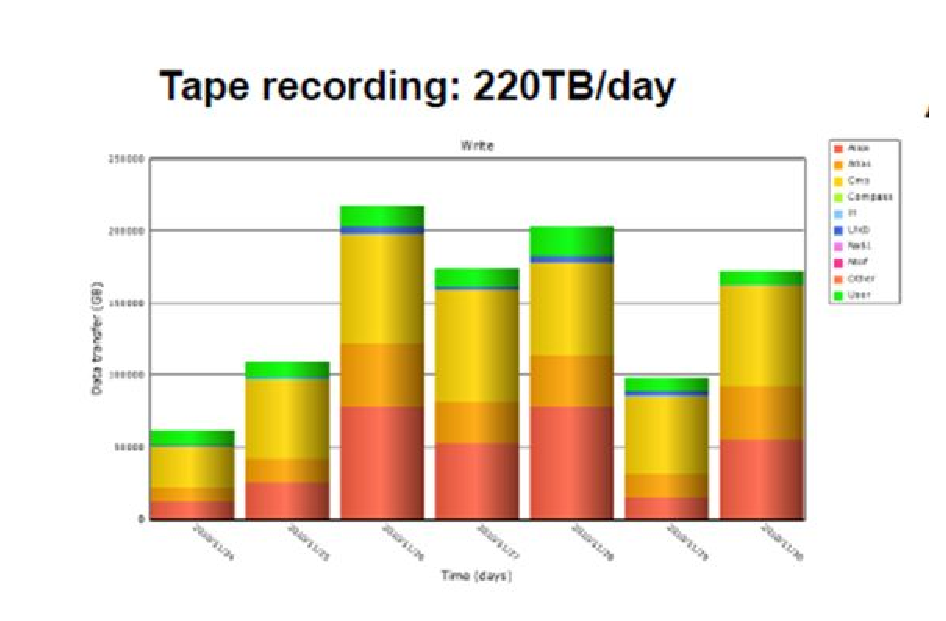
\includegraphics[width=13cm]{fig18.eps} %    ** if .eps don't need extension
\caption{A record in data tape recording: over
220~TB/day}\label{fig18}
\end{figure}


As mentioned in section 2, the mass storage system at the CERN
Tier-0 supported data rates at an average over the year of ~
2.5~GB/s IN with peaks up to 11~GB/s, and data was served at an
average rate of $\sim 7$~GB/s with peaks up to 25~GB/s.

The data processing went on without basic show-stoppers. The
workload management system was able to get about 1 million of jobs
running per day, see Figure~\ref{fig19}, and this load is
gradually going up. This translates into significant amounts of
computer time. Towards the end of 2010 there was a situation when
all of the available job slots at Tier-1s and Tier-2s were often
fully occupied. This has been showing up also during 2011, so the
WLCG collaboration has already now fully used all the available
computing resources. During 2010, the WLCG delivered about
100~CPU-millennia.

%fig19
\begin{figure}[htb] % h-here, t-top, b-bottom
\centering
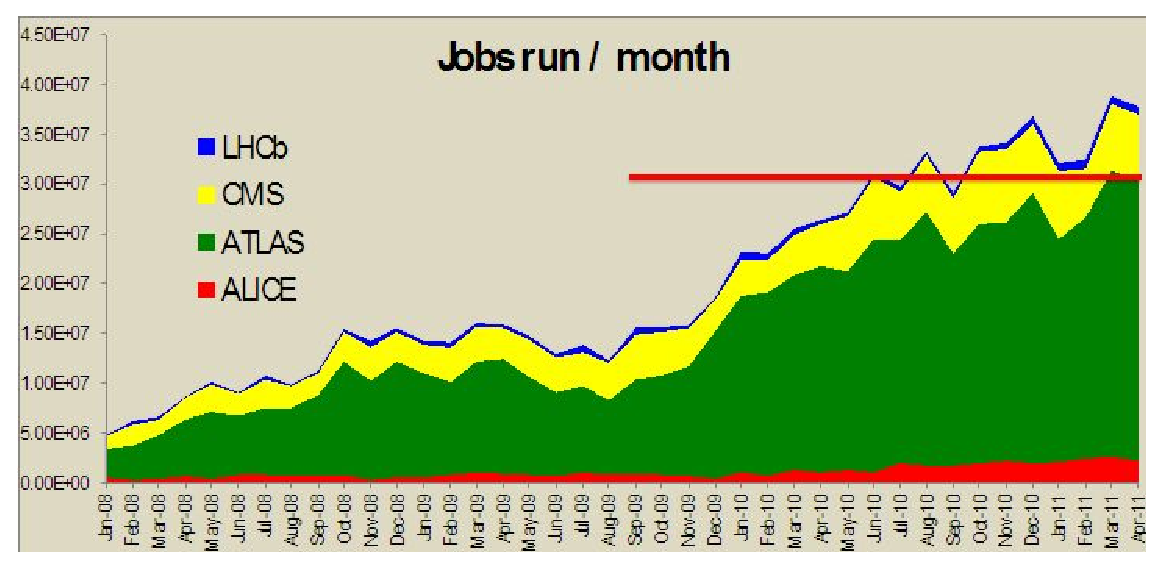
\includegraphics[width=13cm]{fig19.eps} %    ** if .eps don't need extension
\caption{WLCG job profile}\label{fig19}
\end{figure}



As also briefly mentioned in section 2, the WLCG was very successful
concerning the number of individuals really using the grid to
perform their analysis. At the start of the project, there was a
concern that end users will be discouraged from using the grid due
to complexity of its structure and services. But thanks to the
effort of the WLCG and experiments themselves a reasonably simple
access interfaces were developed and the number of end users reached
up to 800 in the large experiments.

The distribution of the delivered CPU power between sites has been
basically according to the original design, but the Tier-2s provided
more than the expected 40\%: it was in fact 50\% or more of the
overall delivery, see section 2. Member countries pledged different
amounts of resources according to their capacities and have been
delivering accordingly.  So the concept of collaborative Grid
resource sharing really works and enables institutes worldwide to
share data, and provide resources to the common goals of the
collaboration.

\subsubsection{Network performance}
%
The key basis for building up a distributed system is the data
transfer infrastructure. The network which the WLCG operates today
is much in advance of what was anticipated in the time of writing
the WLCG TDR. The OPN, see also section 2, started as dedicated
fiber links from CERN to each of the Tier-1s with the throughput 10
Gbit/s. Today, there is a full redundancy in this network with the
original links doubled and with back-up links between Tier-1s
themselves. The OPN is a complicated system with many different
layers of hardware and software and getting it into the current
shape was a difficult task, which evidently paid-off.

The original concerns about the possible network unreliability and
insufficiency were not realized. The network infrastructure relying
on the OPN and the complementary GEANT, US-LHCNet and all the R\&E
national network infrastructures, extensively monitored and
continuously checked with the test transfer jobs, has never been a
problem in the data transfer except for occasional glitches. The
originally estimated sustained transfer rate of 1.3~GB/s from Tier-0
to Tier-1s was reached without problems and exceeded and reached up
to 5~GB/s. Within the OPN, a peak of 70~Gb/s was supported without
any problem during a re-processing campaign of one of the LHC
experiments, see Figure~\ref{fig20}.

%fig20
\begin{figure}[htb] % h-here, t-top, b-bottom
\centering
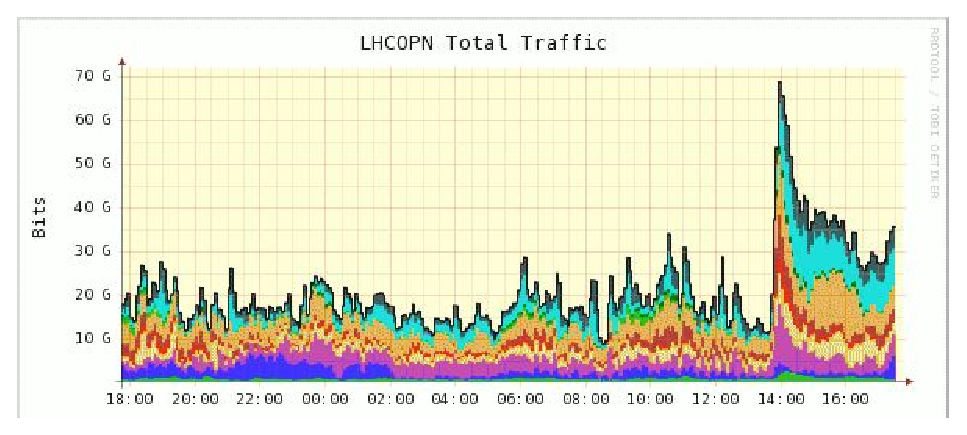
\includegraphics[width=13cm]{fig20.eps} %    ** if .eps don't need extension
\caption{WLCG OPN traffic in 2010 with a peak of 70
Gbit/s}\label{fig20}
\end{figure}



\subsubsection{Concluding remarks - WLCG}
%
The experience from the first year and a half of the LHC data taking
implies that the WLCG has built a truly working grid infrastructure.
The LHC experiments have their own distributed models and have used
the WLCG infrastructure to deliver Physics results within weeks
after the data recording which has never been achieved before. The
fact that a significant numbers of people are doing analysis on the
Grid, that all the resources are being used up to the limits and the
scientific papers are produced with an unprecedented speed is
proving an evident success of the WLCG mission.


\subsection{ALICE performance}
%
To conclude this section, we will briefly summarize the experience
and performance of the ALICE experiment. ALICE started extremely
successfully the processing of the LHC data in 2009: the data
collected during the first collisions delivered by the LHC on
November 23rd (2009) got processed and analyzed so fast that within
one week the article with the results from the first collisions was
accepted for publication as the first ever scientific paper with the
Physics results from the LHC collisions \cite{ALICE_pp}.

\subsubsection{Jobs}
%
During the data taking in 2010, ALICE collected 2.3~PB of raw data,
which represented about 1.2 million of files with the average file
size of 1.9~GB. The data processing chain has been performing
without basic problems.  The Monte Carlo simulation jobs together
with the raw data reconstruction and organized analysis (altogether
the organized production) represented almost 7 millions of
successfully completed jobs, which translates into 0.3 jobs/second.
The chaotic (end user) analysis made for 9 millions of successfully
completed jobs, which represents 0.4 jobs/s, consuming approximately
10\% of the total ALICE CPU resources (the chaotic analysis jobs are
in general shorter than the organized processing jobs).  In total,
there were almost 16 millions of successfully done jobs, which
translates to ~1 job/s and 90 thousands jobs/day.

The running jobs profile got in peaks to 30 thousands of
concurrently running jobs (see Figure~\ref{fig21}) with more than
50\% of the CPU resources delivered by the Tier-2 centers. About
60\% of the total number of jobs represented the end user analysis
(see Figure~\ref{fig22}). In general, the user analysis already in
2010 was a resounding success, with almost 380 people actively using
the Grid. Since the chaotic analysis brings sometimes problems
concerning not completely perfect code resulting, e.g., in a high
memory consumption (cf. section 4), ALICE was running a mixture of
the organized production and end user jobs at all its sites, and
this scenario was working well.

%fig21
\begin{figure}[htb] % h-here, t-top, b-bottom
\centering
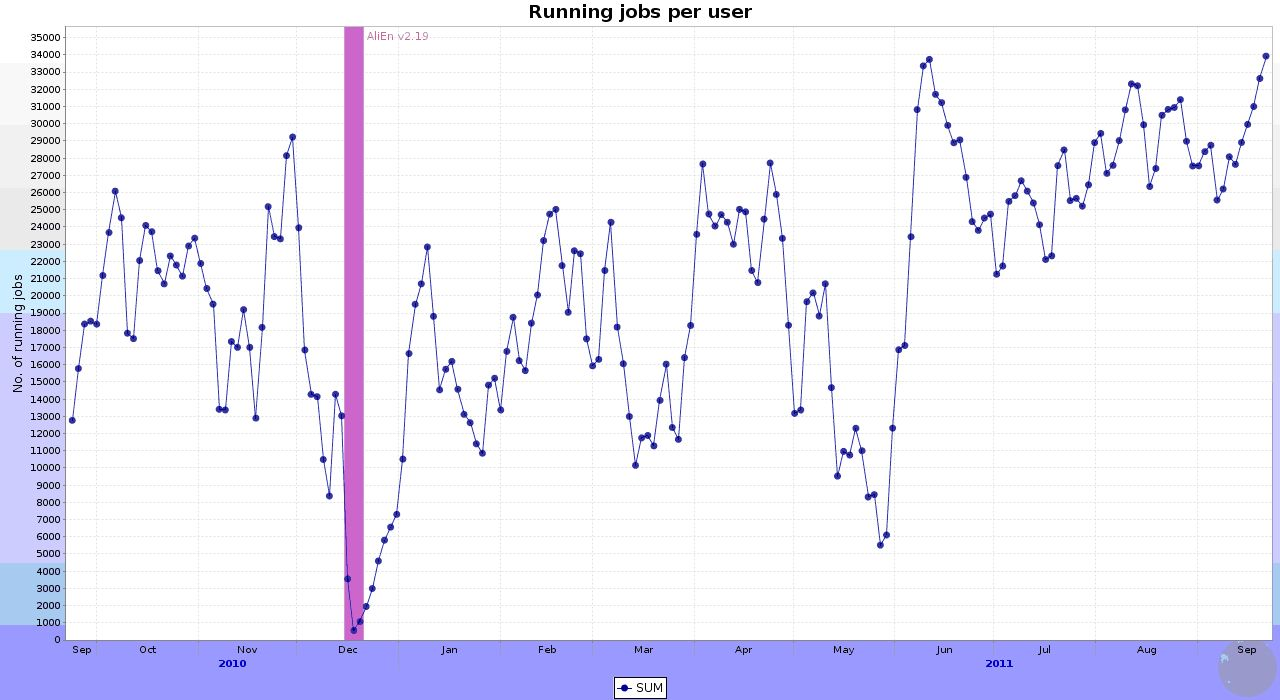
\includegraphics[width=13cm]{fig21.eps} %    ** if .eps don't need extension
\caption{ALICE running jobs profile 2010/2011}\label{fig21}
\end{figure}


%fig22
\begin{figure}[htb] % h-here, t-top, b-bottom
\centering
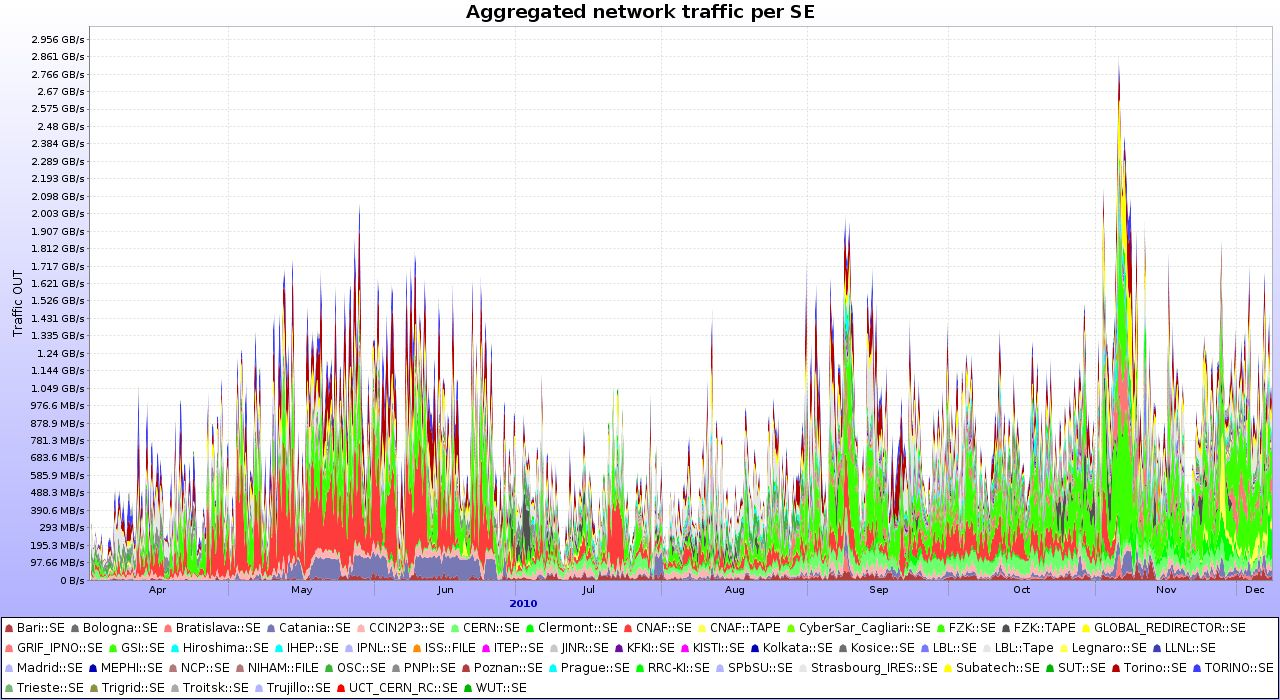
\includegraphics[width=13cm]{fig22.eps} %    ** if .eps don't need extension
\caption{Network traffic OUT by analysis jobs - 2010}\label{fig22}
\end{figure}



\subsubsection{Storage-2010}
%
The distributed storage system endured and was supporting an
enormous load. During 2010/2011, 25.15 PB of data (raw, ESDs, AODs,
Monte Carlo  productions) was written to xrootd Storage Elements
with the speed maximum of 621.1 MB/s. 59.97 PB  of data was read
from the xrootd Storage Elements, with the speed maximum of 1.285
GB/s, see Figure~\ref{fig23}.

%fig23
\begin{figure}[htb] % h-here, t-top, b-bottom
\centering
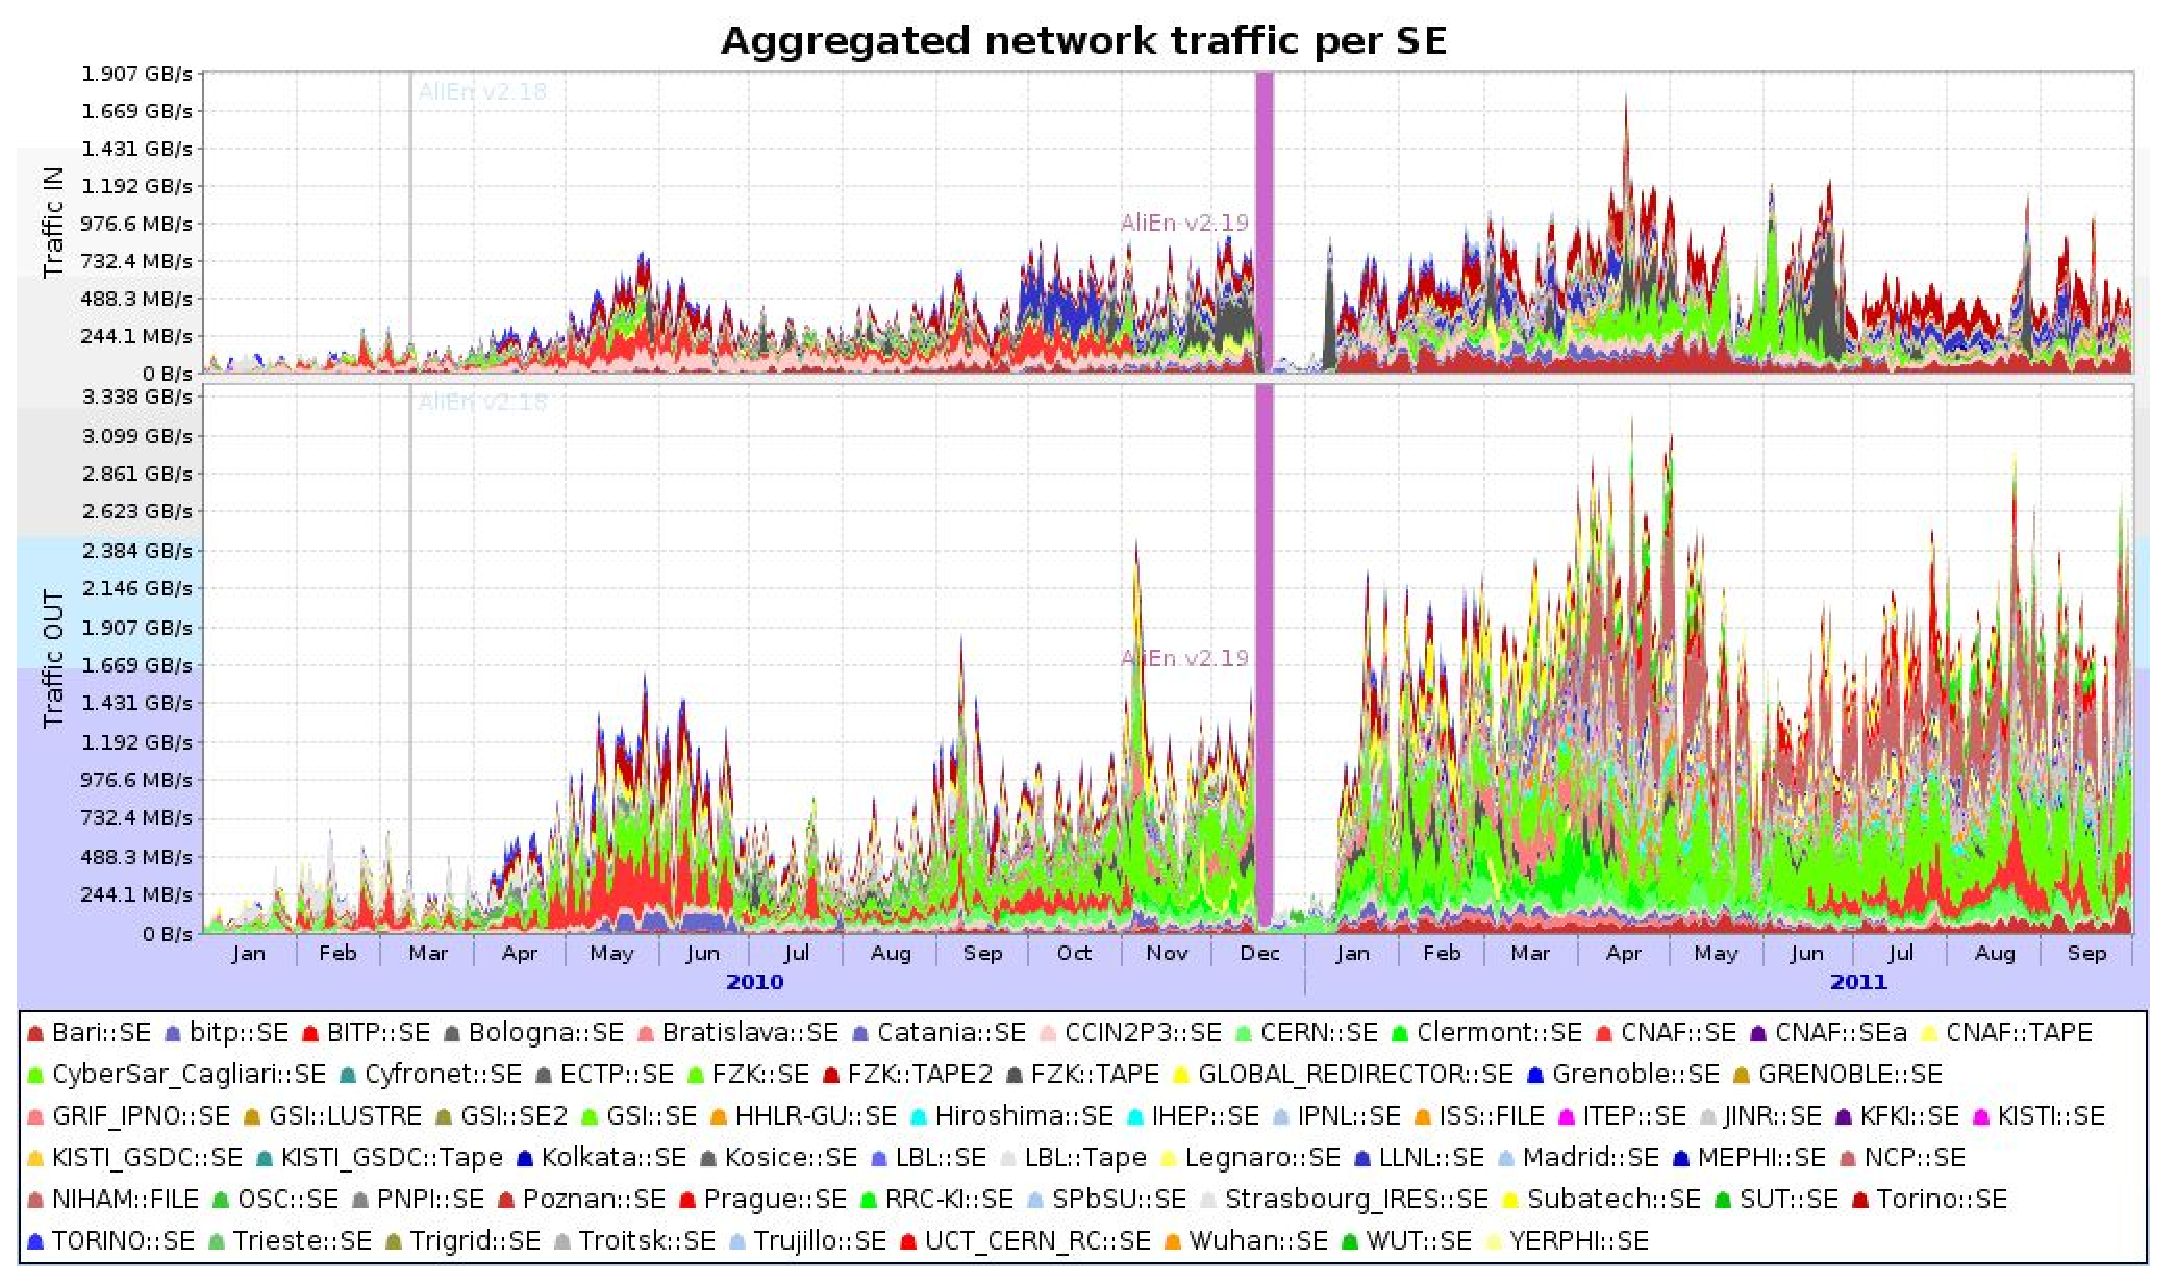
\includegraphics[width=13cm]{fig23.eps} %    ** if .eps don't need extension
\caption{Total network traffic at the ALICE Storage Elements -
2010/2011}\label{fig23}
\end{figure}


\subsubsection{Data taking 2011}
%
Constantly upgrading and extending its hardware resources and
updating the grid software, ALICE continued a successful LHC data
handling campaign in 2011. By September, the total volume of the
collected raw data was almost 1.7~PB with the first reconstruction
pass completed. 2011 was marked by massive user analysis on the
Grid. In May, the most important conference in the Heavy Ion Physics
community, Quark Matter 2011 (QM2011)\cite{QM}, took place and was
preceded by an enormous end user analysis campaign. In average, 6
thousands end-user jobs were running all the time, which represents
almost 30\% of the CPU resources officially dedicated to ALICE (The
number of running jobs is higher than that most of the time due to
use of opportunistic resources). During the week before the QM2011,
there was a peak with 20 thousands of concurrently running end-user
jobs, see Figures~\ref{fig23},\ref{fig24}. The number of active Grid
users reached 411.

%fig24
\begin{figure}[htb] % h-here, t-top, b-bottom
\centering
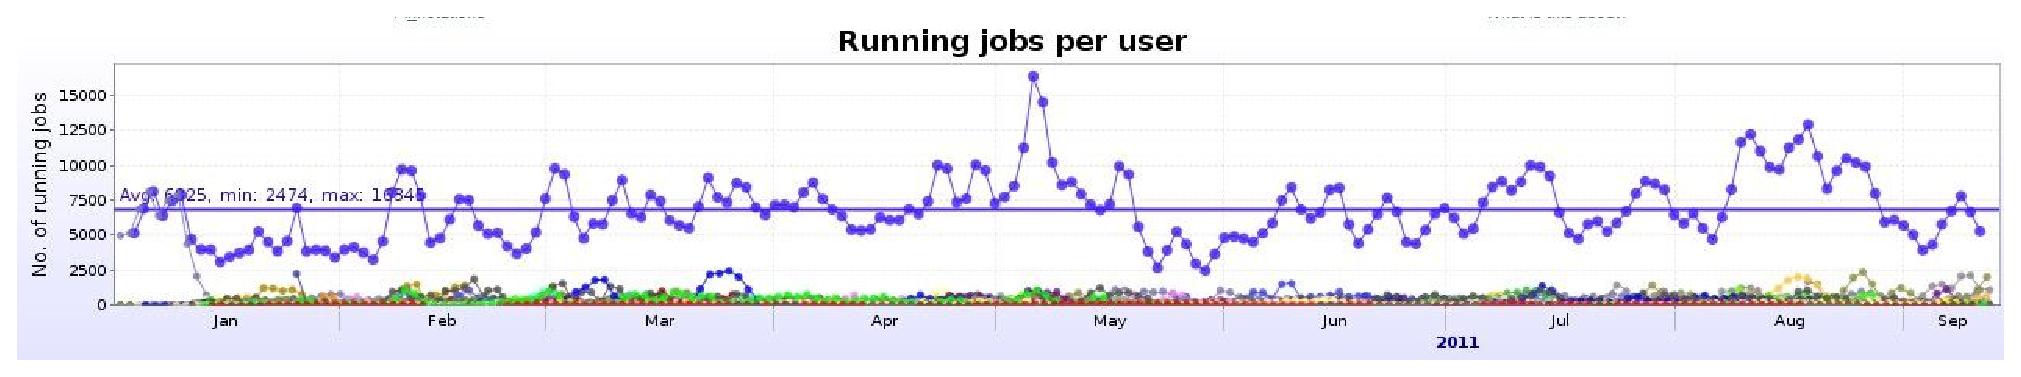
\includegraphics[width=13cm]{fig24.eps} %    ** if .eps don't need extension
\caption{End-user jobs profile - 2011}\label{fig24}
\end{figure}


In total, the ALICE sites were running in average 21 thousands of
jobs with peaks up to 35~thousands (Figure~\ref{fig21}). The
resources ratio remained 50\% delivered by Tier-0 and Tier-1s to
50\% delivered by Tier-2s. Altogether, 69 sites were active in the
operations. The sites' availability and operability kept very stable
throughout the year. The gLite (now EMI) middleware, see section 3,
is mature and only a few changes are necessary. 

In the beginning of the 2011 campaign, there was a concern that the
storage would be saturated. In fact the storage infrastructure was
performing basically without problems supporting the enormous load
from the end-user analysis and was getting ready for the Pb-Pb
operations. The network situation, as was already mentioned for the
WLCG in general, has been excellent and allowed for the operation
scenario where the hierarchical tiered structure got blurred, the
sites of all levels were well interconnected and running a similar
mixture of jobs. As a result, the ALICE Grid in a sense has been
working as a cloud.

\subsection{Concluding remarks - ALICE}
%
In general, similar to the overall characteristics of the WLCG
performance also the ALICE operations and data handling campaigns
were notably successful right from the beginning of the LHC startup,
making the Grid infrastructure operational and supporting a fast
delivery of Physics results. By September 2011, ALICE has published
15 scientific papers with the results from the LHC collisions and
more is on the way. Two papers \cite{alice_mul, alice_pbpb} were marked as ``Suggested
reading'' by the Physical Review Letters editors and the later was
also  selected for the ``Viewpoint in Physics'' by Physical Review
Letters.


%fig25
\begin{figure}[htb] % h-here, t-top, b-bottom
\centering
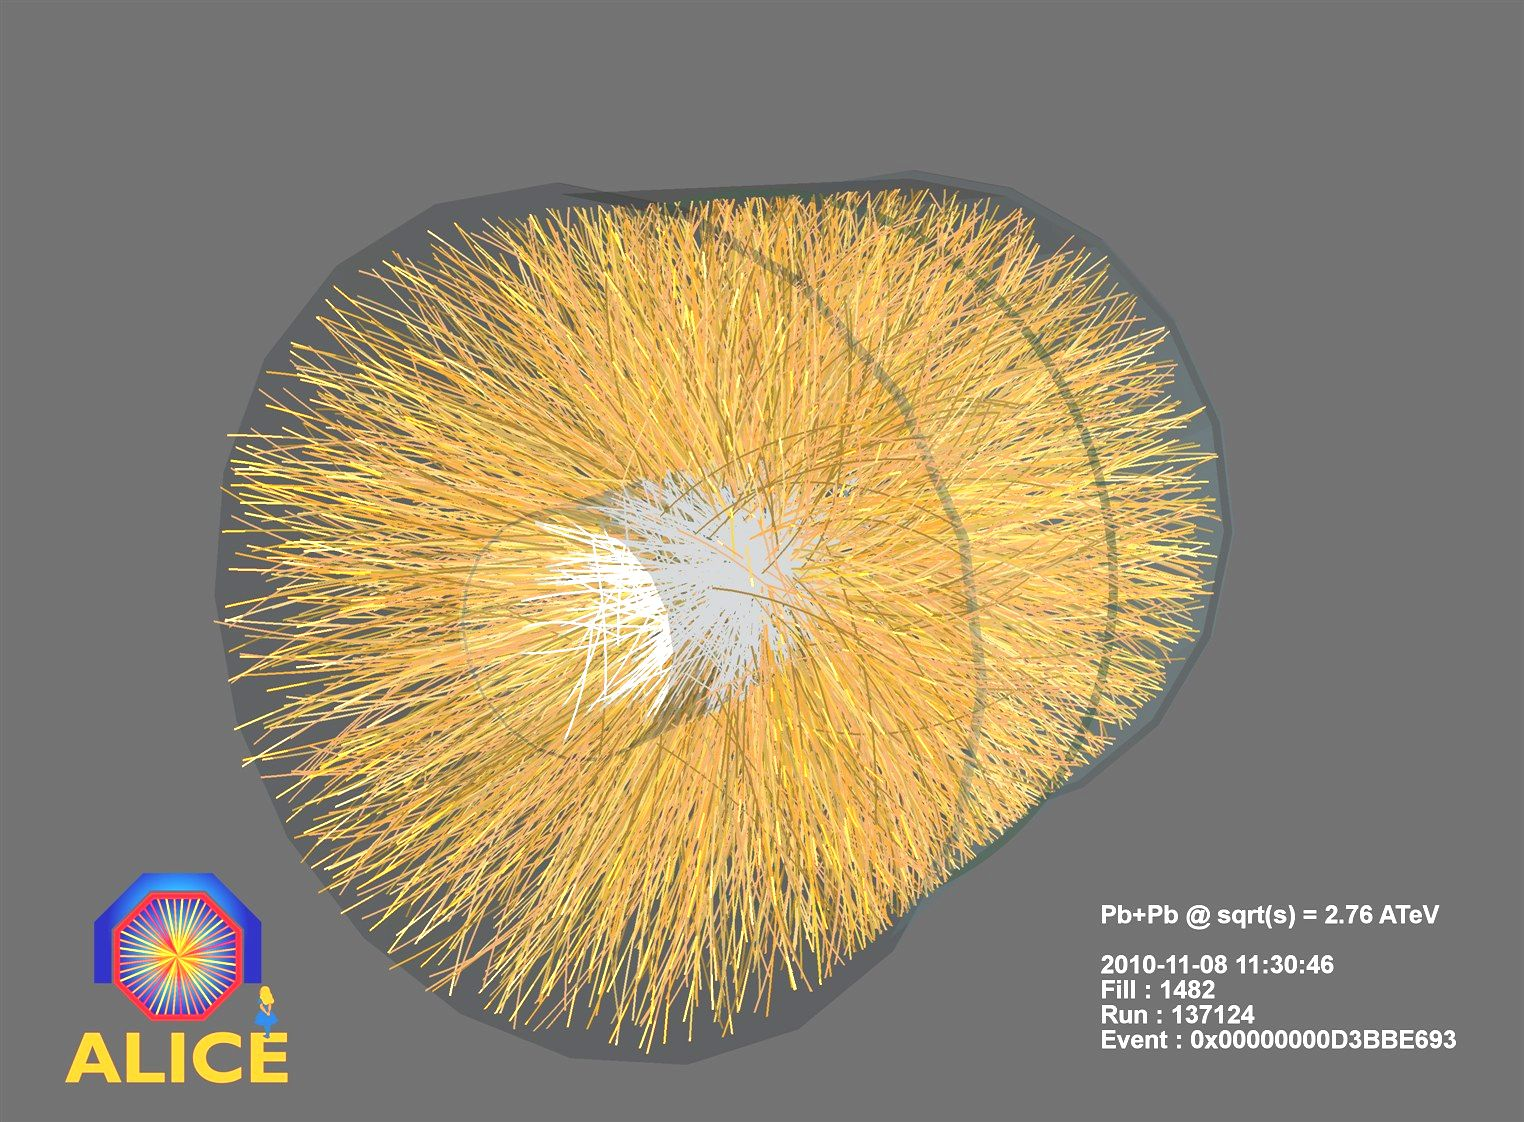
\includegraphics[width=13cm]{fig25.eps} %    ** if .eps don't need extension
\caption{Pb-Pb collision event recorded by ALICE}\label{fig25}
\end{figure}



The full list of the ALICE papers published during 2009-2011 can be
found on \cite{alice_papers}. One of the Pb-Pb collision events recorded by ALICE is
shown on Figure~\ref{fig25}.
